% شروع فصل.
\chapter{فصل مقدمات}
% نوشتن خلاصه‌ی فصل
\begin{summary}
در این فصل ابتدا یک مقدار متن الکی می‌نویسیم و بعد از آن از چند محیط ریاضی استفاده می‌کنیم. در نهایت توضیح می‌دهیم که تصویر برداری چیست و در آخر فصل را با یک بیت شعر به پایان می‌بریم.
\end{summary}

% تعریف بخش.
\section{متن الکی}
لورم ایپسوم متن ساختگی با تولید سادگی نامفهوم از صنعت چاپ و با استفاده از طراحان گرافیک است. چاپگرها و متون بلکه روزنامه و مجله در ستون و سطرآنچنان که لازم است و برای شرایط فعلی تکنولوژی مورد نیاز و کاربردهای متنوع با هدف بهبود ابزارهای کاربردی می باشد. کتابهای زیادی در شصت و سه درصد گذشته، حال و آینده شناخت فراوان جامعه و متخصصان را می طلبد تا با نرم افزارها شناخت بیستری را برای طراحان رایانه ای و فرهنگ پیشرو در زبان فارسی ایجاد کرد. در این صورت می توان امید داشت که تمام و دشواری موجود در ارائه راهکارها و شرایط سخت تایپ به پایان رسد وزمان مورد نیاز شامل حروفچینی دستاوردهای اصلی و جوابگوی سوالات پیوسته اهل دنیای موجود طراحی اساسا مورد استفاده قرار گیرد.

لورم ایپسوم متن ساختگی با تولید سادگی نامفهوم از صنعت چاپ و با استفاده از طراحان گرافیک است. چاپگرها و متون بلکه روزنامه و مجله در ستون و سطرآنچنان که لازم است و برای شرایط فعلی تکنولوژی مورد نیاز و کاربردهای متنوع با هدف بهبود ابزارهای کاربردی می باشد. کتابهای زیادی در شصت و سه درصد گذشته، حال و آینده شناخت فراوان جامعه و متخصصان را می طلبد تا با نرم افزارها شناخت بیستری را برای طراحان رایانه ای و فرهنگ پیشرو در زبان فارسی ایجاد کرد. در این صورت می توان امید داشت که تمام و دشواری موجود در ارائه راهکارها و شرایط سخت تایپ به پایان رسد وزمان مورد نیاز شامل حروفچینی دستاوردهای اصلی و جوابگوی سوالات پیوسته اهل دنیای موجود طراحی اساسا مورد استفاده قرار گیرد.

\section{محیط‌های لاتک}
% تعریف زیربخش برای بخش مذکور.
\subsection{محیط‌های ریاضی}
در این بخش قرار است تا ما چند محیط ریاضی را استفاده کنیم. برای شروع یک تعریف می‌آوریم.
\begin{definition}
این یک تعریف است که البته برای نشان دادن محیط تعریف آمده است.
\end{definition}
و البته اکنون می‌توان یک تعریف دیگر را نیز وارد کرد.
\begin{definition}
البته با این محیط تعریف می‌بینم که شماره‌ها با توجه به بخش افزایش پیدا می‌کنند.
\end{definition}

اکنون که تعاریف لازم را آوردیم، حتی می‌توانیم یک لم را نیز بیاوریم.
\begin{lem}
استفاده از محیط‌های ریاضی‌ای که در فایل \lr{header.tex} تعریف کردیم، به همین صورت است که در اینجا می‌بینید.
\end{lem}
% استفاده از محیط اثبات.
\begin{proof}
اثبات این مبحث را می‌توان با استفاده از آن دید. البته راه‌های دیگری نیز به این منظور وجود دارد، اما این راه بهتر است. پس می‌بینیم که ما از یک محیط اثبات هم استفاده کردیم.
\end{proof}

اکنون به جایی رسیده‌ایم که می‌توانیم از یک محیط فرمول‌نویسی نیز استفاده کنیم. برای مثال یک محیط شماره‌دار
\begin{equation}
% از label برای برچسب‌گذاری برای ارجاعات بعدی استفاده می‌کنیم.
\label{eqn:1:sin_int}
\sin(x) = \int\cos(x)dx + C.
\end{equation}
و می‌بینیم که ما به فرمول \eqref{eqn:1:sin_int} ارجاع می‌دهیم. اکنون یک محیط فرمول بدون شماره را می‌آوریم. قبل از آن دقت کنیم که ما این محیط را با افزودن محیط‌های \lr{ams} در فایل \lr{header.tex} به لاتک اضافه کرده‌ایم که از جامعه‌ی ریاضی آمریکا\LTRfootnote{AMS} به خاطر آماده کردن این محیط تشکر می‌کنیم. نکته‌ی قابل ذکر دیگر قبل از ارائه‌ی محیط بدون شماره این است که ما از محیط \lr{lr} برای وارد کردن محیط انگلیسی در نوشته‌ی فارسی و از \lr{LTRfootnote} برای وارد کردن پانویس انگلیسی استفاده می‌کنیم. این دستورات جز بسته‌ی زی‌پرشین می‌باشند که از آقای وفا خلیقی نیز به خاطر ارائه‌ی این بسته تشکر می‌کنیم. حال محیط ریاضی بدون شماره را استفاده می‌کنیم.
\begin{equation*}
\sin(x) = 1 + x + \mathcal{O}(x^3).
\end{equation*}
واضح است که محیط قبل، بسط تیلور\footnote{بروک تیلور، ۱۶۸۵-۱۷۳۱} تابع $\sin$ را نشان داده است. پس ما در این سطر هم پانوشت فارسی داشتیم و وارد کردن فرمول ریاضی در سطر. به عنوان یک مثال دیگیر می‌توان گفت که $2^3 = 8$، البته در مورد این فرمول همه‌ی ریاضی‌دانان متفق‌القول نیستند.

در حال حاضر محیط ریاضی دیگری به ذهنم نمی‌رسید. اگر محیطی را نیاز دارید، لطفا توضیحات آنرا در این پست وبلاگم \lr{http://meysampg.blog.ir/post/38/} ارسال کنید و یا به \lr{meysam@pourganji.ir} ایمیل بفرستید.

\subsection{تصویر برداری در متن}
\label{ssec:usegraphics}
در این بخش ما افزودن تصویر برداری به متن را نشان می‌دهیم. ابتدا یک تصویر نشان می‌دهیم
\begin{figure}[!h]
\centerline{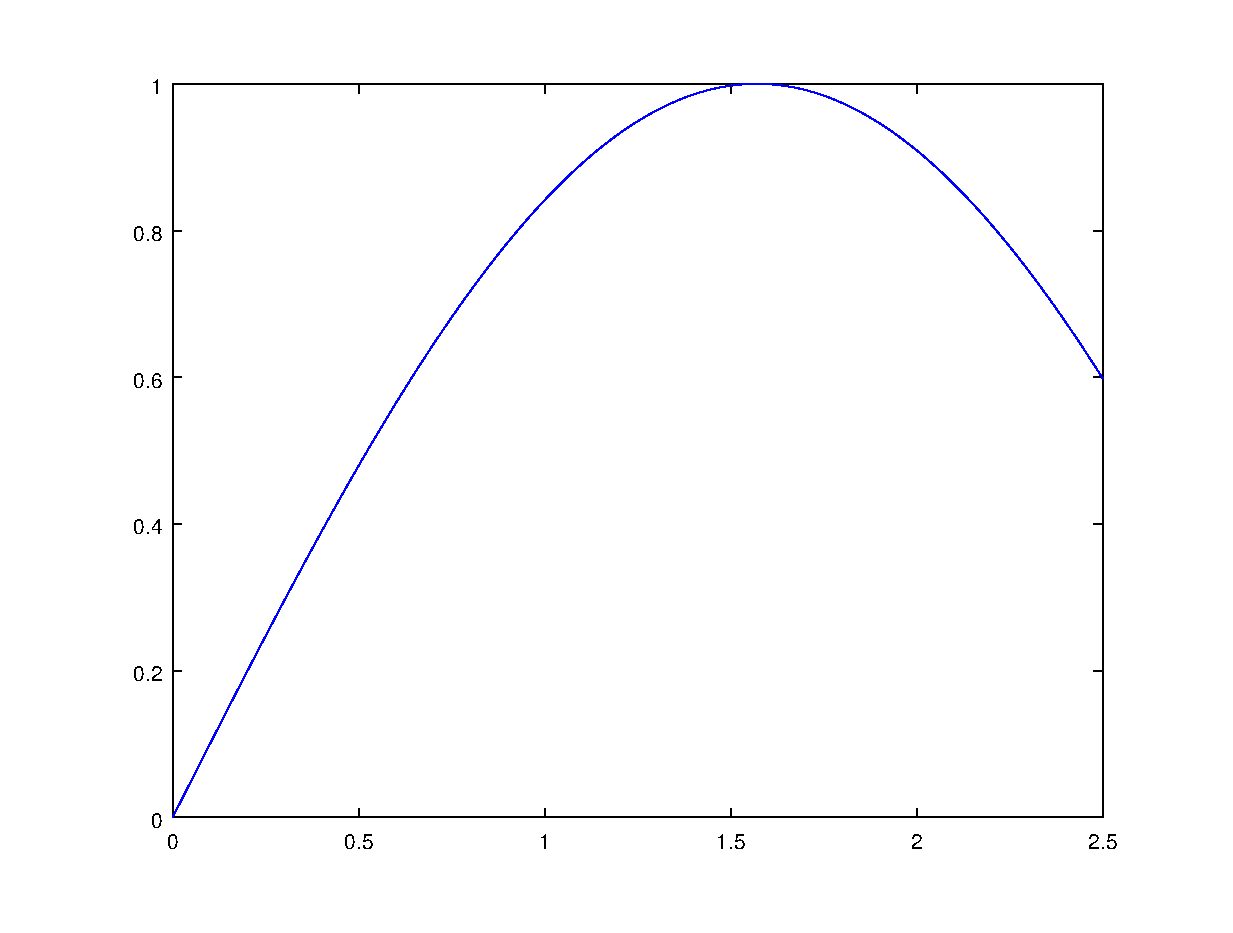
\includegraphics[scale=.45]{sin}}
\caption{تصویر تابع $\sin$.}
\label{fig:1:sin}
\end{figure}

دقت کنیم که ما مسیر فایل‌های تصویر را پوشه‌ی \lr{figures} تعریف کرده‌ایم و اگر آن را باز کنید، می‌بینید که یک فایل \lr{sin.eps} در آن وجود دارد که ما در تصویر \ref{fig:1:sin} از آن استفاده کرده‌ایم. دقت به یک نکته‌ی ریز ولی همچنی مهم لازم است که در محیط‌هایی که از دستور \lr{caption} استفاده می‌کنید -مثل محیط بالا- همیشه اول دستور \lr{caption} را آورده و بعد از آن از دستور \lr{label} استفاده کنید. در غیراینصورت در ارجاعت به برچسب، لاتک نمی‌تواند شماره‌ی ارجاع را تشخیص دهد.

حال دو تصویر را در یک محیط نشان می‌دهیم. یکی همان تصویر تابع سینوس است و دیگری تصویر حاصل از دستور $\cos(x)\times\sin(x)$ در اکتاو (یا متلب).

\begin{figure}[h]
\centering
% محیط subfigure با فراخوانی بسته‌ی subcaption به لاتک اضافه می‌شود.
\begin{subfigure}[b]{.45\textwidth}
	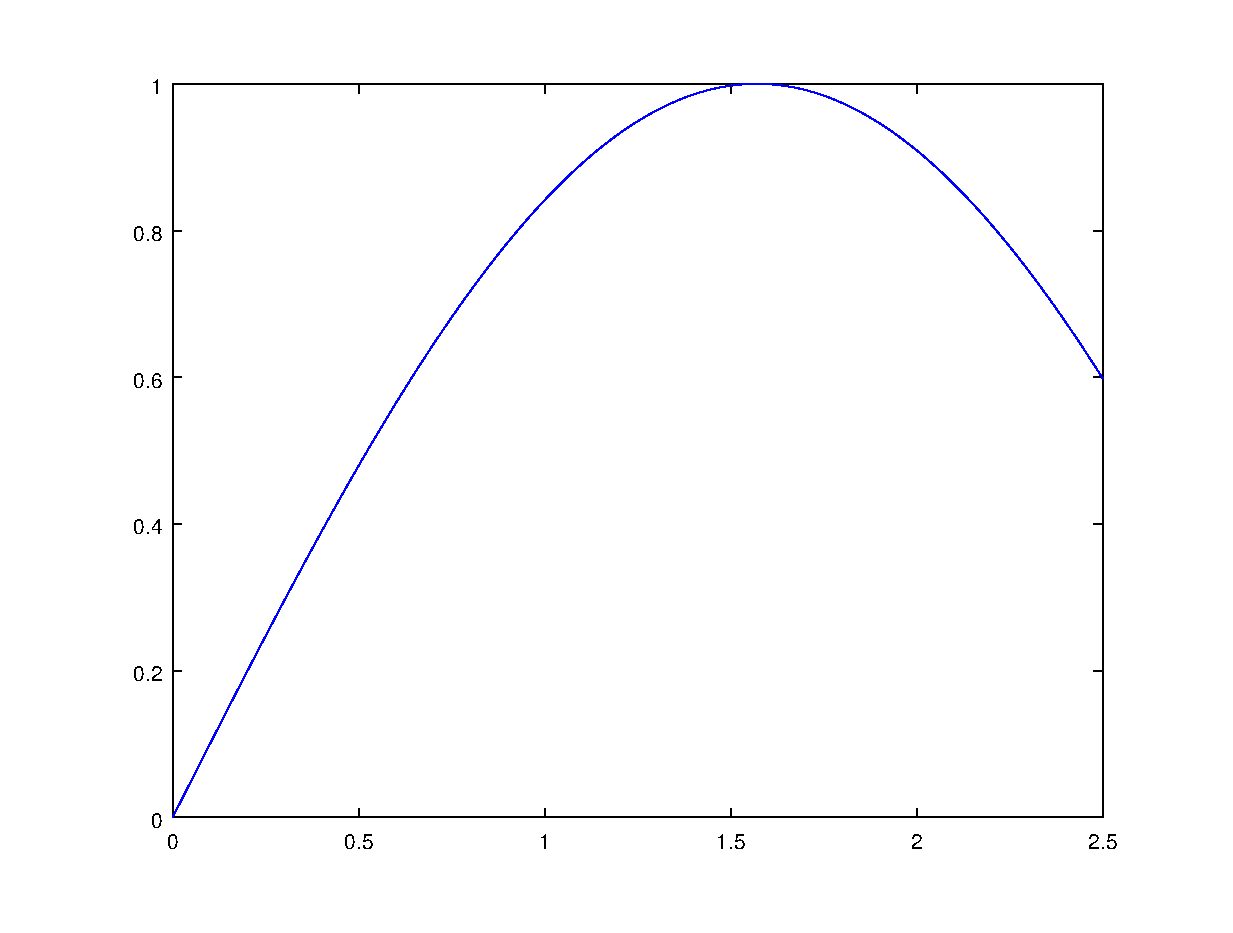
\includegraphics[width=\textwidth]{sin}
	\caption{تصویر تابع $\sin$ به عنوان یک تصویر.}
	\label{fig:1:sin_subfig}
\end{subfigure}
\begin{subfigure}[b]{.45\textwidth}
	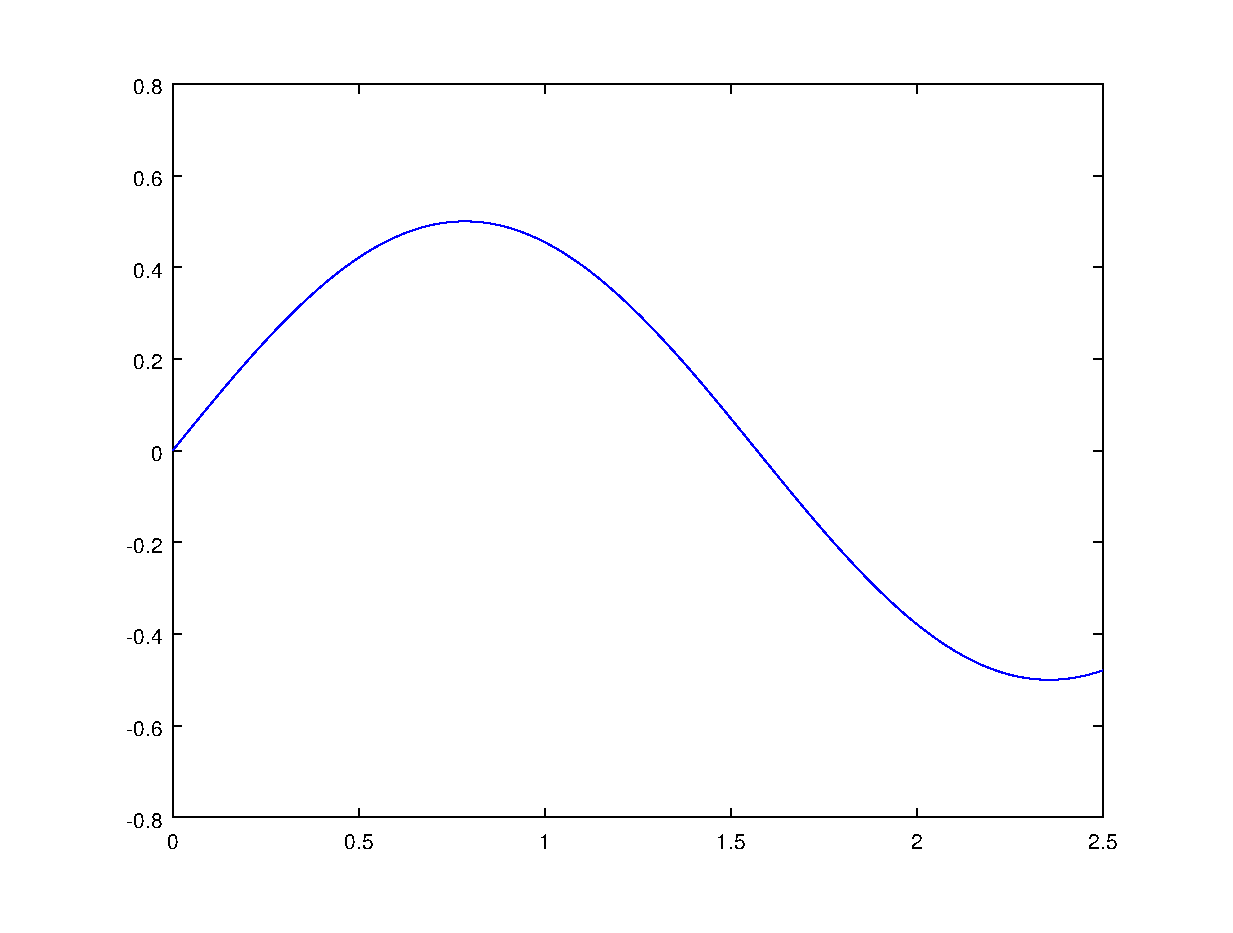
\includegraphics[width=\textwidth]{sincos}
	\caption{تصویر تابع $\sin(x)\times\cos(x)$.}
	\label{fig:1:sincos_subfig}
\end{subfigure}
\caption{تصویر دو تابع.}
\label{fig:1:anotherfig}
\end{figure}

طبیعی است که ما بتوانیم به مجموعه‌ی تصاویر \ref{fig:1:anotherfig} و یا یکی از آن تصاویر، مثلا تصویر \ref{fig:1:sincos_subfig} ارجاع بدهیم. می‌بینیم که همه چی به خوبی کار می‌کند.

\section{تصاویر برداری}
در بخش \ref{ssec:usegraphics} دیدیم که می‌توان از تصاویر برداری در متن لاتک استفاده نمود، اما یک سوال اساسی باقی می‌ماند: «تصویر برداری چیست و چگونه می‌توان آنرا ساخت؟». به صورت خلاصه گرافیک برداری دارای این خاصیت است که با بزرگنمایی تصویر، کیفیت آن از دست نمی‌رود. به منظور آشنایی خوانندگان گرامی با شیوه‌ی ارجاع دادن، برای مطالعه‌ی بیشتر منابع \cite{wiki:vecGraphFa} و \cite{wiki:vecGraphEn} در دسترس است. لطفا فایل \lr{ref.bib} را باز کنید تا طریقه‌ی استفاده از آنها را ببینید. در صورتی که به مراجع خود چیزی اضافه کردید، طریقه‌ی رندر فایل خروجی به صورت زیر است:

\begin{latin}
\lstinputlisting[language=bash]{codes/render_file.bash}
\end{latin}

همچنین پسندیده است تا فایل \lr{chapter01.tex} را باز کنید و ببینید که ما چگونه کد متلب را در اینجا وارد کرده‌ایم.

در نهایت سوال دوم یعنی طریقه‌ی ساخت تصویر برداری را در فصل بعد توضیح خواهیم داد.

\section{یک بیت شعر}
می‌فرماید:
\begin{center}
در میان انجمن یک آن افتاد شال از سرش\\
از همان شب مجمع دیوانگان آغاز شد
\end{center}
در اینجا فصل اول را تمام می‌کنیم و فصل دوم را شروع می‌کنیم.